\documentclass{article}
\usepackage{lingmacros}
\usepackage[danish]{babel}
\usepackage{enumitem}
\usepackage{lmodern}
\usepackage[utf8]{inputenc}
\usepackage[T1]{fontenc}
\usepackage{color}
\usepackage{amssymb}
\usepackage{listings}
\usepackage{listingsutf8}
\usepackage{color} %red, green, blue, yellow, cyan, magenta, black, white
\definecolor{mygreen}{RGB}{28,172,0} % color values Red, Green, Blue
\definecolor{mylilas}{RGB}{170,55,241}
\lstset{literate=
  {æ}{{\ae}}{1} 
  {å}{{\aa}}{1} 
  {ø}{{\o}}{1} }
\usepackage{graphicx}
\usepackage[export]{adjustbox}
\usepackage{fullpage}
\lstset{basicstyle=\ttfamily,breaklines=true}
% \lstset{framextopmargin=50pt,frame=bottomline}
\lstset{
% numbers=left, 
% numberstyle=\small, 
% numbersep=8pt, 
frame = single, 
language=Pascal, 
framexleftmargin=15pt}
\usepackage[T1]{fontenc}
\usepackage[hidelinks]{hyperref}
 \usepackage{tree-dvips}
% \usepackage{biblatex}
% \usepackage[style=verbose,backend=bibtex]{biblatex}
% \bibliography{oeve1dsb.bib}
% \usepackage{sagetex}
\usepackage{amsmath}
% \usepackage{newpxtext,newpxmath}
\usepackage{courier}
\linespread{1.5}
\makeatletter
\renewcommand*\env@matrix[1][*\c@MaxMatrixCols c]{%
  \hskip -\arraycolsep
  \let\@ifnextchar\new@ifnextchar
  \array{#1}}
\makeatother
\title{E4DSA\\ Case projekt 2 – audio IIR notch filter}
\author{Team 8}
\def\emptyline{\vspace{12pt}}

\begin{document}
%\newcommand{\includecode}[2][c]{\lstinputlisting[caption=#2, escapechar=, style=custom#1]{#2}<!---->}
\lstset{language=Matlab,%
    %basicstyle=\color{red},
    breaklines=true,%
    morekeywords={matlab2tikz},
    keywordstyle=\color{blue},%
    morekeywords=[2]{1}, keywordstyle=[2]{\color{black}},
    identifierstyle=\color{black},%
    stringstyle=\color{mylilas},
    commentstyle=\color{mygreen},%
    showstringspaces=false,%without this there will be a symbol in the places where there is a space
    % numbers=left,%
    % numberstyle={\tiny \color{black}},% size of the numbers
    % numbersep=9pt, % this defines how far the numbers are from the text
    emph=[1]{for,end,break},emphstyle=[1]\color{red}, %some words to emphasise
    %emph=[2]{word1,word2}, emphstyle=[2]{style},    
  }
\maketitle
\tableofcontents
\newpage

\section{Data analyse}
\label{sec:Data analyse}

\subsection{Matlab kode}
\label{sec:matlab1}

\begin{lstlisting}
n = 0:N-1;
load('vejecelle_data.mat');
x = vejecelle_data;

figure
plot(n,x), grid
xlabel('n'), ylabel('x(n)'), title('hele signalet DC-signal')
\end{lstlisting}

Det første tiltag der blev lavet for at løse opgaven var at se signalet fysisk, dette blev derfor gjort ved først at loade signalet ind via load funktionen, navnet på signalet blev x, og denne blev plottet, plottet ses på figur 
\begin{figure}[h!]
  \centering
  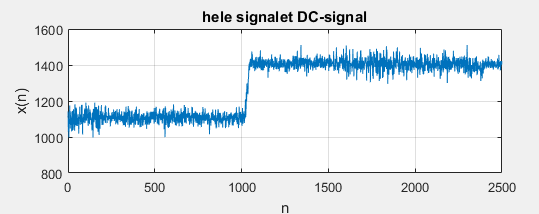
\includegraphics[width=0.8\textwidth]{rod/startsignal.png}
  \caption{hele signalet}
  \label{fig:helesignal}
\end{figure}

Der ses på billede \ref{fig:helesignal} hvordan selve signalet ser ud, nu kan der påbegyndes analyse af dette, der ønskes analyse af henholdsvist første halvdel, hvilket er vurderet fra 0 til 1000 samples, samt anden halvdel som er vurderet til 1050 til 2500 samples.

\begin{lstlisting}
%% MA-filter (ikke-rekursivt) for første del
M = 16;    % filterkoefficienter
hMA = 1/M*ones(1,M); % MA-filter, filterkoefficienter

hMA_imp_resp  = hMA;                        % impulsrespons
hMA_step_resp = filter(hMA,1,ones(1,2*M));  % steprespons
L_MA_trans_resp = M-1;                      % længde af transientrespons
HMA1 = fft(hMA,Nfft);                        % frekvensrespons

yMA1 = filter(hMA,1,x1);            % filtrerer inputsignal for første del
yMA2 = filter(hMA,1,x2);            % filtrerer inputsignal for anden del

var_x1 = var(x1(M:N1));    % varians i 1 signal i del efter transientrespons
var_yMA1 = var(yMA1(M:N1));% varians i 1 signal i del efter transientrespons

var_x2 = var(x2(M:N2));    % varians i 2 signal i del efter transientrespons
var_yMA2 = var(yMA2(M:N2));% varians i 2 signal i del efter transientrespons
\end{lstlisting}

følgende kode sætter filterkoefficienter op, udregner impulsrespons, stepresons, længde af transientrespons, frekvensrespons, samt lægger MA filteret på de to del signaler, og afslutningsvist udregner variansen ud med funktionen var, således dette kan plottes

\begin{lstlisting}
%% --- plotting for første signal ---
figure('name', 'første MA-filter')
subplot(2,6,1:3)
plot(n1,x1), grid
xlabel('n'), ylabel('x(n)'), title('første del af DC-signal')

subplot(2,6,4:6)
histogram(x1)
title('histogram')

subplot(2,6,7:10)
plot(n1,x1), grid, hold on
plot(n1,yMA1,'linewidth',2)
xlabel('n'), ylabel('x(n)'), title(['MA-filter, M = ' num2str(M)])
legend('input','output')

subplot(2,6,11:12)
text(0,0.5,...
    {['første MA-filter, M = ' num2str(M)],...
     ['Transientrespons: ' num2str(L_MA_trans_resp) ' samples'],...
     ['Støjeffekt i inputsignal (varians):  ' num2str(var_x1)],...
     ['Støjeffekt i outputsignal (varians): ' num2str(var_yMA1)],...
     ['Reduktion i støjeffekt: ' num2str((var_x1/var_yMA1)) ' gange'],...
     ['Reduktion i støjeffekt: ' num2str(10*log10(var_x1/var_yMA1)) ' dB']})
 axis off
\end{lstlisting}

Da koden for plots af første del af signalet, er det samme som plotsene for anden del, med den undtagelse x1 samt N1 er udskiftet med x2 og N2, redegøres der kun for første del.
første plot er signalet for sig selv, dette kommer til at udgøre halvdelen af øverste skærm da subplottet har 2*6 vinduer.
herefter anvendes funktionen histogram til at plotte histogrammet.
3 plot er signalet henholdsvist før og efter MA filteret er tilsat, således dæmpningen som konsekvens af dette filter bliver tydeligtgjort.
Sidste subplot er udregning af transientresponset, hvor tidligere oprettede variabel L_MA_trans_resp bliver omskrevet til et character array via num2str funktionen.
herefter printes støjeffekten for de to signaler, num2str er igen anvendt, og her printes ligeledes tidligere udregnet variabler var_x1 samt var_yMA1.
disse bliver divideret med hinanden for at få reduktionen i støjeffekten herefter, og afslutningsvist hvor mange gange dette bliver dæmpet henholdsvist både i decimal værdi, samt med hvor mange decibel.

\subsection{plots}
\label{sec:plots}

\begin{figure}[h!]
  \centering
  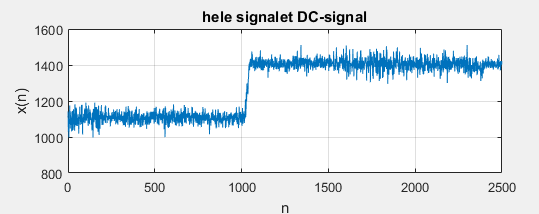
\includegraphics[width=0.8\textwidth]{rod/startsignal.png}
  \caption{starsignal}
  \label{fig:2signaler}
\end{figure}

figur \ref{fig:2signaler} viser plots af de to isolerede dele af oprindelige signal der ønskes analyseret, der kan her ses middelværdien på første del af signalet er på 1100 hertz (anden del er på 1400)

\begin{figure}[h!]
  \centering
  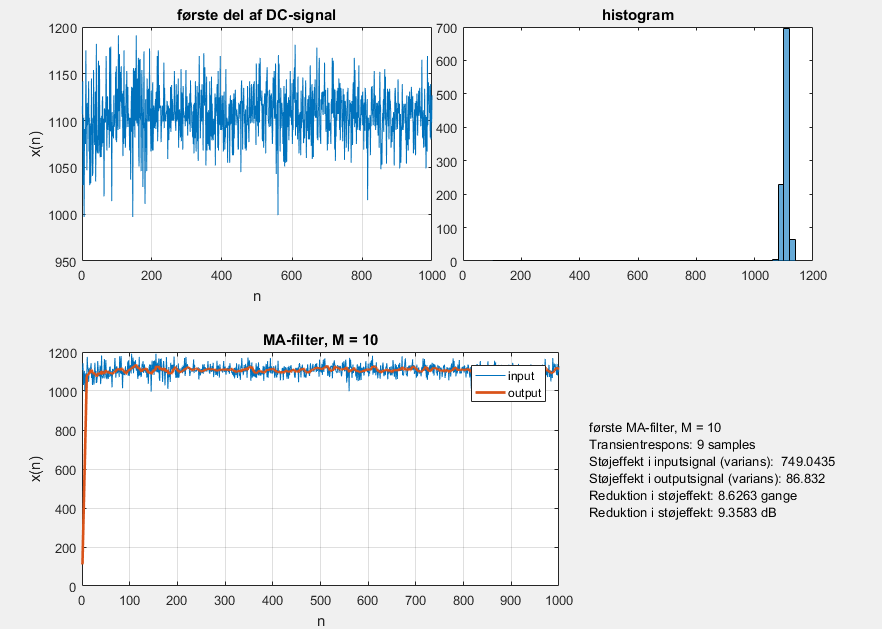
\includegraphics[width=0.8\textwidth]{rod/1MAfilter.png}
  \caption{plots af første signal}
  \label{fig:1signalplot}
\end{figure}

figur \ref{fig:1signalplot} viser plots af første del af signalet, her ses på histogrammet der er en middelværdi på ca 1100, dette passer meget godt overens med plottet af frekvenserne i signalet, da 1100 også ser ud til at være ca. midten her.
på 3 subplot ses det oprindelige signal igen med blå, her er den røde linje output signalet efter MA filteret er tilsat, dette er nu noget mere udjævnet, hvilket leder til konklusionen at der må være en del normaltfordelt støj på signalet.

\subsection{afstand imellem bit niveauer i gram}
\label{sec:afstand}

\section{Design af midlingsfilter}
\label{sec:Design}

\subsection{forsøg med midlingsfiltre}
\label{sec:forsøg}

\subsection{beregning af max FIR længde}
\label{sec:beregning}

\subsection{Alfa's betydning}
\label{sec:alfa}

\section{Systemovervejelser}
\label{sec:Systemovervejelser}

\end{document}
